\documentclass[10pt, aspectratio=169]{beamer}
\usepackage{../beamer_theme_408}
\title{408考研零基础 --- 计算机网络}
\subtitle{4-11 路由算法}
\author{}
\date{}
\begin{document}

\begin{frame}{本节目标}
    \begin{enumerate}
        \item 理解静态路由与动态路由的区别
        \item 掌握距离向量算法（RIP）的原理及问题
        \item 掌握链路状态算法（OSPF）的原理及特点
        \item 了解BGP边界网关协议的基本作用
    \end{enumerate}
\end{frame}

\begin{frame}{路由算法概述}
    \begin{columns}[t]
        \column{0.5\textwidth}
        \textbf{静态路由}
        \begin{itemize}
            \item 管理员手动配置路由表
            \item 简单、安全、可预测
            \item 无法适应拓扑变化
            \item 适合小型网络
        \end{itemize}
        \column{0.5\textwidth}
        \textbf{动态路由}
        \begin{itemize}
            \item 路由器自动计算路由
            \item 适应拓扑变化
            \item 适合大型复杂网络
            \item 分为距离向量和链路状态
        \end{itemize}
    \end{columns}
    \vspace{0.5em}
    \begin{center}
        \begin{tikzpicture}[>=stealth]
            \node[draw,fill=blue!10] at (-1.5,0) {路由算法};
            \node[draw,fill=green!10] at (1.5,0.7) {静态};
            \node[draw,fill=red!10] at (1.5,-0.7) {动态};
            \draw[->] (-0.5,0) -- (1,0.7);
            \draw[->] (-0.5,0) -- (1,-0.7);
            \node[draw,fill=yellow!10] at (3.5,0) {距离向量(RIP)};
            \node[draw,fill=yellow!10] at (3.5,-1.4) {链路状态(OSPF)};
            \draw[->] (2.2,0) -- (2.8,0);
            \draw[->] (2.2,-0.7) -- (2.8,-1.4);
        \end{tikzpicture}
    \end{center}
\end{frame}

\begin{frame}{距离向量算法 --- RIP协议}
    \begin{block}{核心思想}
        每个路由器维护一张路由表，记录到所有目的网络的距离（跳数）和下一跳。
        \textbf{邻居之间交换整张路由表}，每个邻居传自己的路由表。
    \end{block}
    \vspace{0.3em}
    \begin{columns}[t]
        \column{0.5\textwidth}
        \textbf{Bellman-Ford方程}
        \[
        d_x(y) = \min\{c(x,v) + d_v(y)\}
        \]
        \begin{itemize}
            \item $d_x(y)$：从$x$到$y$的最短距离
            \item $c(x,v)$：从$x$到邻居$v$的代价
            \item $d_v(y)$：邻居$v$到$y$的距离
        \end{itemize}
        \column{0.5\textwidth}
        \textbf{RIP特点}
        \begin{itemize}
            \item 跳数$\le 15$，16表示不可达
            \item 每30秒广播一次路由表
            \item UDP端口520
            \item 慢收敛
        \end{itemize}
    \end{columns}
\end{frame}

\begin{frame}{距离向量算法 --- 工作过程}
    \begin{center}
        \begin{tikzpicture}[>=stealth, node distance=1.5cm]
            \node[draw,circle,minimum size=1cm] (A) {A};
            \node[draw,circle,minimum size=1cm,right=of A] (B) {B};
            \node[draw,circle,minimum size=1cm,right=of B] (C) {C};
            \node[draw,circle,minimum size=1cm,right=of C] (D) {D};
            \draw (A) -- node[above]{1} (B);
            \draw (B) -- node[above]{1} (C);
            \draw (C) -- node[above]{1} (D);
        \end{tikzpicture}
    \end{center}
    \vspace{0.3em}
    \begin{columns}[t]
        \column{0.5\textwidth}
        \textbf{A初始路由表}
        \begin{itemize}
            \item A: 0, 本地
            \item B: 1, B
        \end{itemize}
        \vspace{0.3em}
        \textbf{收到B的路由表后}
        \begin{itemize}
            \item C: 2, B
            \item D: 3, B
        \end{itemize}
        \column{0.5\textwidth}
        \textbf{更新规则}
        \begin{enumerate}
            \item 收到邻居$v$的路由表
            \item 对每个目的网络$y$：
            \item 新距离 $= c(x,v) + d_v(y)$
            \item 若新距离 $<$ 原距离，更新
        \end{enumerate}
    \end{columns}
\end{frame}

\begin{frame}{RIP --- 慢收敛与计数到无穷}
    \begin{block}{问题}
        当网络拓扑发生变化（如链路断开），RIP可能需要很长时间才能收敛。
    \end{block}
    \begin{center}
        \begin{tikzpicture}[>=stealth]
            \node[draw,circle,minimum size=0.8cm] (A) {A};
            \node[draw,circle,minimum size=0.8cm,right=of A] (B) {B};
            \node[draw,circle,minimum size=0.8cm,right=of B] (C) {C};
            \draw (A) -- node[above]{1} (B);
            \draw (B) -- node[above]{1} (C);
            \draw[red,thick] (B) -- node[above]{断开！} (C);
        \end{tikzpicture}
    \end{center}
    \vspace{0.3em}
    \begin{itemize}
        \item C到A原路径：C$\to$B$\to$A，距离2
        \item C$\to$B断开后，B从A学到C可达（B误以为A到C有路径）
        \item B告诉C：我到A的距离是2 $\Rightarrow$ C以为到A的距离是3
        \item C告诉B：我到A的距离是3 $\Rightarrow$ B更新为4
        \item 恶性循环，计数到16才停止（16=不可达）
    \end{itemize}
    \vspace{0.3em}
    \begin{exampleblock}{解决方法}
        水平分割（Split Horizon）：从某接口学到的路由，不向该接口通告。
    \end{exampleblock}
\end{frame}

\begin{frame}{链路状态算法 --- OSPF协议}
    \begin{block}{核心思想}
        每个路由器收集全网的链路状态信息（LS），形成一致的网络拓扑图，独立运行Dijkstra算法计算最短路径树。
    \end{block}
    \vspace{0.3em}
    \begin{columns}[t]
        \column{0.5\textwidth}
        \textbf{工作步骤}
        \begin{enumerate}
            \item 发现邻居，测量链路代价
            \item 构造LSP（链路状态分组）
            \item 泛洪LSP给所有路由器
            \item 每个路由器构建全网拓扑
            \item 运行Dijkstra计算最短路径
        \end{enumerate}
        \column{0.5\textwidth}
        \textbf{OSPF特点}
        \begin{itemize}
            \item \textbf{触发更新}，收敛快
            \item 适合大型网络
            \item IP协议号89
            \item 支持认证
            \item 区域划分提高扩展性
        \end{itemize}
    \end{columns}
\end{frame}

\begin{frame}{Dijkstra最短路径算法}
    \begin{block}{算法步骤}
        \begin{enumerate}
            \item 初始化：源节点距离为0，其他为$\infty$
            \item 从未确定节点中选择距离最小的节点$u$
            \item 将$u$标记为已确定
            \item 更新$u$的邻居距离：$d(v) = \min\{d(v), d(u) + c(u,v)\}$
            \item 重复2-4步直到所有节点确定
        \end{enumerate}
    \end{block}
    \vspace{0.3em}
    \begin{exampleblock}{示例}
        \begin{center}
            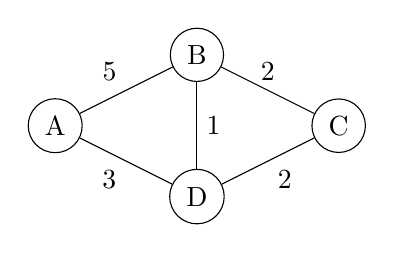
\begin{tikzpicture}[>=stealth, scale=0.9]
                \node[draw,circle] (A) at (0,0) {A};
                \node[draw,circle] (B) at (2,1) {B};
                \node[draw,circle] (C) at (4,0) {C};
                \node[draw,circle] (D) at (2,-1) {D};
                \draw (A) -- node[above left]{5} (B);
                \draw (A) -- node[below left]{3} (D);
                \draw (B) -- node[above]{2} (C);
                \draw (B) -- node[right]{1} (D);
                \draw (C) -- node[below right]{2} (D);
            \end{tikzpicture}
        \end{center}
    \end{exampleblock}
\end{frame}

\begin{frame}{OSPF --- 区域划分}
    \begin{center}
        \begin{tikzpicture}[>=stealth]
            \node[draw,circle,minimum size=1.2cm,fill=red!20] (area0) at (0,0) {Area 0\\骨干区域};
            \node[draw,circle,minimum size=1cm,fill=blue!20] (area1) at (-2.5,-2) {Area 1};
            \node[draw,circle,minimum size=1cm,fill=blue!20] (area2) at (2.5,-2) {Area 2};
            \node[draw,circle,minimum size=1cm,fill=blue!20] (area3) at (0,2) {Area 3};
            \draw (area0) -- (area1);
            \draw (area0) -- (area2);
            \draw (area0) -- (area3);
            \node[below] at (-2.5,-2.8) {普通区域};
            \node[below] at (0,-0.8) {所有区域必须与Area 0相连};
        \end{tikzpicture}
    \end{center}
    \vspace{0.3em}
    \begin{itemize}
        \item \textbf{骨干区域（Area 0）}：所有非骨干区域必须与其相连
        \item \textbf{普通区域}：通过ABR（区域边界路由器）连接骨干区域
        \item \textbf{优点}：限制LSA泛洪范围，减少路由计算量
    \end{itemize}
\end{frame}

\begin{frame}{距离向量 vs 链路状态}
    \begin{table}
        \centering
        \begin{tabular}{|c|c|c|}
            \hline
            \textbf{特性} & \textbf{距离向量（RIP）} & \textbf{链路状态（OSPF）} \\
            \hline
            交换内容 & 整张路由表 & 链路状态信息 \\
            算法 & Bellman-Ford & Dijkstra \\
            收敛速度 & 慢 & 快 \\
            跳数限制 & 15跳 & 无 \\
            更新方式 & 定期(30s) & 触发 \\
            复杂性 & 简单 & 复杂 \\
            适用规模 & 小型网络 & 大型网络 \\
            \hline
        \end{tabular}
    \end{table}
    \vspace{0.5em}
    \begin{itemize}
        \item RIP：实现简单，易出现计数到无穷问题
        \item OSPF：收敛快，适合大型网络，支持层次划分
    \end{itemize}
\end{frame}



\begin{frame}{本节总结}
    \begin{enumerate}
        \item 静态路由（手动配置）vs 动态路由（自动计算）
        \item 距离向量算法（RIP）：Bellman-Ford方程，邻居交换路由表，跳数$\le$15，慢收敛、计数到无穷
        \item 链路状态算法（OSPF）：收集全网LS，Dijkstra计算，触发更新，收敛快，区域划分
        \item BGP：自治系统间路由，路径向量算法，TCP 179
    \end{enumerate}
\end{frame}

\end{document}
